\documentclass[letterpaper, 11 pt]{article}
\usepackage{amssymb, latexsym, amsmath, amsthm, graphicx, amsthm,alltt,color, listings,multicol,xr-hyper,hyperref,aliascnt,enumitem}
\usepackage{xfrac}

\usepackage{parskip}
\usepackage[,margin=0.7in]{geometry}
\setlength{\textheight}{8.5in}

\usepackage{epstopdf}

\DeclareGraphicsExtensions{.eps}
\usepackage{tikz}


\usepackage{tkz-euclide}
%\usetkzobj{all}
\tikzstyle geometryDiagrams=[rounded corners=.5pt,ultra thick,color=black]
\colorlet{penColor}{black} % Color of a curve in a plot


\usepackage{subcaption}
\usepackage{float}
\usepackage{fancyhdr}
\usepackage{pdfpages}
\newcounter{includepdfpage}
\usepackage{makecell}


\usepackage{currfile}
\usepackage{xstring}




\graphicspath{  
{./otherDocuments/}
}

\author{Claire Merriman}
\newcommand{\classday}[1]{\def\classday{#1}}

%%%%%%%%%%%%%%%%%%%%%
% Counters and autoref for unnumbered environments
% Not needed??
%%%%%%%%%%%%%%%%%%%%%
\theoremstyle{plain}


\newtheorem*{namedthm}{Theorem}
\newcounter{thm}%makes pointer correct
\providecommand{\thmname}{Theorem}

\makeatletter
\NewDocumentEnvironment{thm*}{o}
 {%
  \IfValueTF{#1}
    {\namedthm[#1]\refstepcounter{thm}\def\@currentlabel{(#1)}}%
    {\namedthm}%
 }
 {%
  \endnamedthm
 }
\makeatother


\newtheorem*{namedprop}{Proposition}
\newcounter{prop}%makes pointer correct
\providecommand{\propname}{Proposition}

\makeatletter
\NewDocumentEnvironment{prop*}{o}
 {%
  \IfValueTF{#1}
    {\namedprop[#1]\refstepcounter{prop}\def\@currentlabel{(#1)}}%
    {\namedprop}%
 }
 {%
  \endnamedprop
 }
\makeatother

\newtheorem*{namedlem}{Lemma}
\newcounter{lem}%makes pointer correct
\providecommand{\lemname}{Lemma}

\makeatletter
\NewDocumentEnvironment{lem*}{o}
 {%
  \IfValueTF{#1}
    {\namedlem[#1]\refstepcounter{lem}\def\@currentlabel{(#1)}}%
    {\namedlem}%
 }
 {%
  \endnamedlem
 }
\makeatother

\newtheorem*{namedcor}{Corollary}
\newcounter{cor}%makes pointer correct
\providecommand{\corname}{Corollary}

\makeatletter
\NewDocumentEnvironment{cor*}{o}
 {%
  \IfValueTF{#1}
    {\namedcor[#1]\refstepcounter{cor}\def\@currentlabel{(#1)}}%
    {\namedcor}%
 }
 {%
  \endnamedcor
 }
\makeatother

\theoremstyle{definition}
\newtheorem*{annotation}{Annotation}
\newtheorem*{rubric}{Rubric}

\newtheorem*{innerrem}{Remark}
\newcounter{rem}%makes pointer correct
\providecommand{\remname}{Remark}

\makeatletter
\NewDocumentEnvironment{rem}{o}
 {%
  \IfValueTF{#1}
    {\innerrem[#1]\refstepcounter{rem}\def\@currentlabel{(#1)}}%
    {\innerrem}%
 }
 {%
  \endinnerrem
 }
\makeatother

\newtheorem*{innerdefn}{Definition}%%placeholder
\newcounter{defn}%makes pointer correct
\providecommand{\defnname}{Definition}

\makeatletter
\NewDocumentEnvironment{defn}{o}
 {%
  \IfValueTF{#1}
    {\innerdefn[#1]\refstepcounter{defn}\def\@currentlabel{(#1)}}%
    {\innerdefn}%
 }
 {%
  \endinnerdefn
 }
\makeatother

\newtheorem*{scratch}{Scratch Work}


\newtheorem*{namedconj}{Conjecture}
\newcounter{conj}%makes pointer correct
\providecommand{\conjname}{Conjecture}
\makeatletter
\NewDocumentEnvironment{conj}{o}
 {%
  \IfValueTF{#1}
    {\innerconj[#1]\refstepcounter{conj}\def\@currentlabel{(#1)}}%
    {\innerconj}%
 }
 {%
  \endinnerconj
 }
\makeatother

\newtheorem*{poll}{Poll question}
\newtheorem{tps}{Think-Pair-Share}[section]


\newenvironment{obj}{
	\textbf{Learning Objectives.} By the end of class, students will be able to:
		\begin{itemize}}
		{\!.\end{itemize}
		}

\newenvironment{pre}{
	\begin{description}
	}{
	\end{description}
}


\newcounter{ex}%makes pointer correct
\providecommand{\exname}{Homework Problem}
\newenvironment{ex}[1][2in]%
{%Env start code
\problemEnvironmentStart{#1}{Homework Problem}
\refstepcounter{ex}
}
{%Env end code
\problemEnvironmentEnd
}

\newcommand{\inlineAnswer}[2][2 cm]{
    \ifhandout{\pdfOnly{\rule{#1}{0.4pt}}}
    \else{\answer{#2}}
    \fi
}


\ifhandout
\newenvironment{shortAnswer}[1][
    \vfill]
        {% Begin then result
        #1
            \begin{freeResponse}
            }
    {% Environment Ending Code
    \end{freeResponse}
    }
\else
\newenvironment{shortAnswer}[1][]
        {\begin{freeResponse}
            }
    {% Environment Ending Code
    \end{freeResponse}
    }
\fi

\let\question\relax
\let\endquestion\relax

\newtheoremstyle{ExerciseStyle}{\topsep}{\topsep}%%% space between body and thm
		{}                      %%% Thm body font
		{}                              %%% Indent amount (empty = no indent)
		{\bfseries}            %%% Thm head font
		{}                              %%% Punctuation after thm head
		{3em}                           %%% Space after thm head
		{{#1}~\thmnumber{#2}\thmnote{ \bfseries(#3)}}%%% Thm head spec
\theoremstyle{ExerciseStyle}
\newtheorem{br}{In-class Problem}

\newenvironment{sketch}
 {\begin{proof}[Sketch of Proof]}
 {\end{proof}}


\newcommand{\gt}{>}
\newcommand{\lt}{<}
\newcommand{\N}{\mathbb N}
\newcommand{\Q}{\mathbb Q}
\newcommand{\Z}{\mathbb Z}
\newcommand{\C}{\mathbb C}
\newcommand{\R}{\mathbb R}
\renewcommand{\H}{\mathbb{H}}
\newcommand{\lcm}{\operatorname{lcm}}
\newcommand{\nequiv}{\not\equiv}
\newcommand{\ord}{\operatorname{ord}}
\newcommand{\ds}{\displaystyle}
\newcommand{\floor}[1]{\left\lfloor #1\right\rfloor}
\newcommand{\legendre}[2]{\left(\frac{#1}{#2}\right)}



%%%%%%%%%%%%




\newcommand{\ord}{\operatorname{ord}}

\title{Week 14--MATH 4573 Elementary Number Theory}

\begin{document}

\maketitle
%\tableofcontents
%%%%%%%%%%%%%%%%%%%%%%%%%
%%%%%%%%%%%%%%%%%%%%%%%%%
\section{Monday, April 12: Finishing the proof of Quadratic Reciprocity and Pythagorean Triples}
%%%%%%%%%%%%%%%%%%%%%%%%%%

%%%%%%%%%%%%%%%%%%%%%%%%%%
\subsection{Finishing the proof of Quadratic Reciprocity (15 minutes)}
%%%%%%%%%%%%%%%%%%%%%%%%%%
Let's review what where we left off: 

We are trying to show that $\left(\frac{p}{q}\right)\left(\frac{q}{p}\right)=(-1)^{\frac{(p-1)}{2}\frac{(q-1)}{2}}$.

From the lemma from last Wednesday, we know that for \[N_1=\sum_{j=1}^{(p-1)/2}\left\lfloor\frac{jq}{p}\right\rfloor, N_2=\sum_{j=1}^{(p-1)/2}\left\lfloor\frac{jp}{q}\right\rfloor\] then \[\left(\frac{q}{p}\right)=(-1)^{N_1}, \left(\frac{p}{q}\right)=(-1)^{N_2}.\]

We are trying to then show that $N_1+N_2=\frac{(p-1)}{2}\frac{(q-1)}{2}$.

We assumed that $p>q$ and drew the rectangle 
$O=(0,0), A=\left(\frac{p-1}{2},0\right), B=\left(\frac{p-1}{2},\frac{q-1}{2}\right),$ and $C=\left(0,\frac{q-1}{2}\right)$, like in the graphic below:

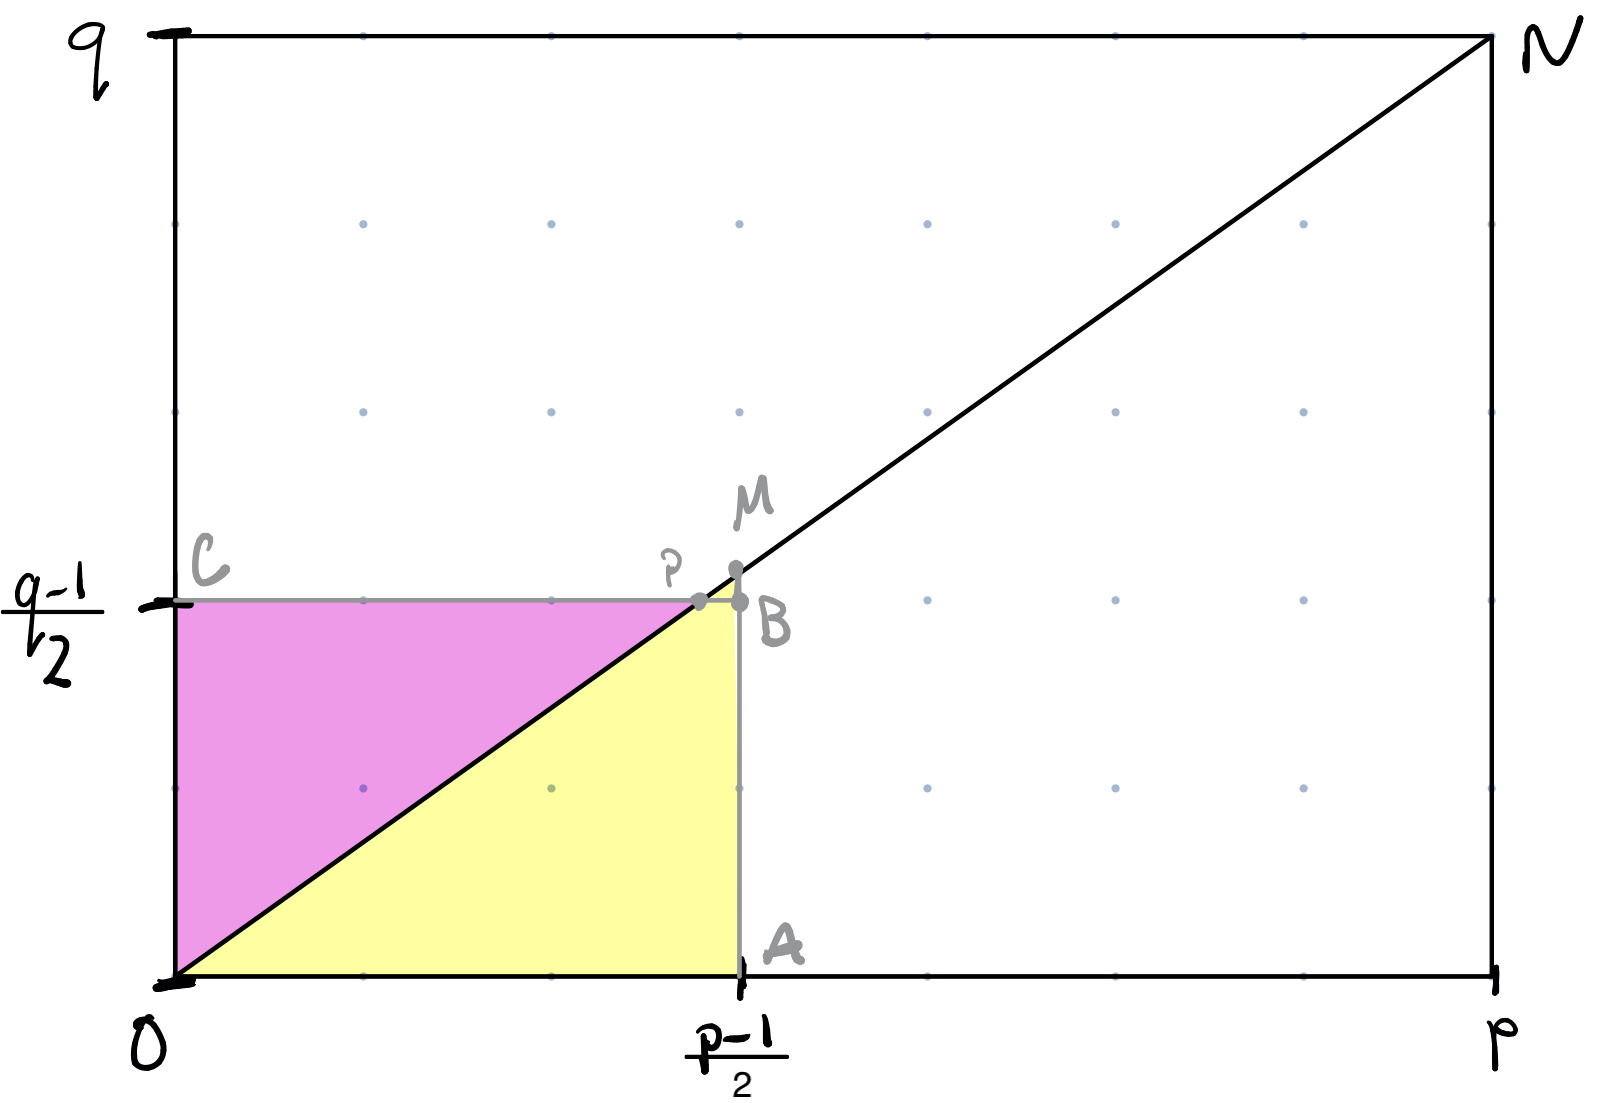
\includegraphics[width=\textwidth]{lattice}

We showed that here are $\frac{(p-1)}{2}\frac{(q-1)}{2}$. Our goal is to show that there are $N_1$ lattice points in the pink area and $N_2$ lattice points in the yellow. Last class, we showed that the triangle $OMA$ and the quadrilateral $OPBA$ have the same number of lattice points. It is slightly easier to count points for the triangle, so we do that.

\begin{proof}
To find $N_1$, the number of lattice points in $OPC$, not including those on $OC$, we count how many lattice points on the line $y=j$ are to the left of $ON$ for $j=1,2,\dots,\frac{q-1}{2}$. Another was of saying this is for each $j$, we want the number of nonnegative integers less than    {$\frac{jp}{q}$}

Thus, we have for each $j$, there are 
{$\left\lfloor\frac{jp}{q}\right\rfloor$} 
lattice points in $OPC$. Thus, in total there are $N_1=\displaystyle\sum_{j=1}^{(q-1)/2}\left\lfloor\frac{jp}{q}\right\rfloor$ lattice points in $OPC$.


To find $N_2$, we use a similar counting method on $OAM$. Now, we count the lattice points on $x=j$ for $j=1,2,\dots,\frac{p-1}{2}$. Thus, for each $j$, we want the number of nonnegative integers less than     {$\frac{jq}{p}$}. Thus, we have for each $j$, there are    {$\left\lfloor\frac{jq}{p}\right\rfloor$}
lattice points in $OPC$. Thus, in total there are  $N_2=  \displaystyle\sum_{j=1}^{2
}\left\lfloor\frac{jq}{p}\right\rfloor$ lattice points in $OMA$.
From the previous Lemma, $\left(\frac{p}{q}\right)=(-1)^{N_1}$ and $\left(\frac{q}{p}\right)=(-1)^{N_2}$. Thus, 
\begin{align*}
 \left(\frac{p}{q}\right)\left(\frac{p}{q}\right)&=(-1)^{N_1} (-1)^{N_2} \\
 &=(-1)^{N_1+N_2}\\
&=(-1)^{\frac{p-1}{2}\frac{q-1}{2}}
\end{align*}
with the result from the April 7 reading assignment.
\end{proof}

Quadratic reciprocity means that determining all quadratic residues (perfect squares) modulo an odd prime is a finite problem. In terms of Legendre symbol, this is finding all $a$ where $\left(\frac{a}{p}\right)=1$ for a given $p$. For example, when $p=11$, we can check all positive integers $a$. However, what about the reverse? Quadratic reciprocity allows us to find all odd primes $p$ where $\left(\frac{11}{p}\right)=1,$ even though there are infinitely many odd primes. This idea is also on Homework 12, Short Proofs.


%%%%%%%%%%%%%%%%%%%%%%%%%
\subsection{Announcements (5 min)}
%%%%%%%%%%%%%%%%%%%%%%%%%
We are going to leave quadratic reciprocity for nonprimes for independent study. Hopefully, if you need this information in the future, you have gained some of the skill of reading and working through mathematics. 

In the interest of moving away from super technical topics, we are going to skip arithmetic functions and the M\"obius inversion formula. This will make the last week a bit of a grab bag of number theory topics, but I want to move into Diophantine equations, which are more concrete. This will also keep us looking at things that are vaguely geometric.

We also are going to take a slightly different approach than the book, and use Pythagorean triples as our motivating example. This means we will do parts of Chapter 11 before Chapter 10.


%%%%%%%%%%%%%%%%%%%%%%%%%%
\subsection{Linear Diophantine equation review (10 minutes)}
%%%%%%%%%%%%%%%%%%%%%%%%%%

\begin{defn}
 A \emph{Diophantine equation} is any equation in one or more variables to be solved in the integers.
\end{defn}
\begin{defn}
 Let $a_1,a_2,\dots,a_n,b\in\mathbb{Z}$ with $a_1,a_2,\dots,a_n$ not zero. A Diophantine equation of the form \[a_1x_1+a_2x_2+\cdots+a_nx_n=b\] is a \emph{linear Diophantine equation in the $n$ variable $x_1,\dots,x_n$}.
\end{defn}

The participation assignment classifies linear Diophantine equations in one variable.

The question of whether there are solutions to Diophantine equations becomes harder when there is more than one variable. Then next step is to classify Diophantine equations in two variables.

\begin{thm}[Theorem 1.13]
 Let $ax+by=c$ be a linear Diophantine equation in the variables $x$ and $y$. Let $d=\gcd(a,b)$. If $d\nmid c$, then the equation has no solutions; if $d\mid c$, then the equation has infinitely many solutions. Furthermore, if $x_0,y_0$ is a particular solution of the equation, then all solution are given by $x=x_0+\frac{b}{d}n$ and $y=y_0-\frac{a}{d}n$ where $n\in\mathbb{Z}$.
\end{thm}
\begin{br}[7 minutes]
Find all solutions to $803x+154y=11$.
\end{br}
%%%%%%%%%%%%%%%%%%%%%%%%%%
\subsection{Nonlinear Diophantine equations (5 minutes)}
%%%%%%%%%%%%%%%%%%%%%%%%%%
\begin{defn}
 A Diophantine equation is \emph{nonlinear} if it is not linear.
\end{defn}

\begin{example}
 
\begin{enumerate}
 \item The Diophantine equation $x^2+y^2=z^2$ is our next section. Solutions are called Pythagorean triples.
 \item Let $n\in\mathbb{Z}$ with $n\geq 3$. The Diophantine equation $x^n+y^n=z^n$ is the subject of the famous Fermat's Last Theorem. We will also prove one case of this.
 \item Let $n\in\mathbb{Z}$. The Diophantine equation $x^2+y^2=n$ tells us which integers can be represented as the sum of two squares.
 \item Let $d,n\in\mathbb{Z}$. The Diophantine equation $x^2-dy^2=n$ is known as Pell's equation.
\end{enumerate}
\end{example}

Sometimes we can use congruences to show that a particular nonlinear Diophantine equation has no solutions. 

\begin{example}
 Prove that $3x^2+2=y^2$ is not solvable.
 
 Assume that there is a solution. Then any solution to the Diophantine equation is also a solution to the congruence $3x^2+2\equiv y^2 \mod 3$, which implies $2\equiv y^2 \mod 3$, which we know is false. Thus there are no integer solutions to $3x^2+2=y^2$.
\end{example}

Note: viewing the same equation modulo 2 says $x^2\equiv y^2 \mod 2$, which does not give us enough information to prove a solution does not exist.
%%%%%%%%%%%%%%%%%%%%%%%%%
\section{Wednesday, April 14: Pythagorean triples and Fermat's Last Theorem}
%%%%%%%%%%%%%%%%%%%%%%%%%%
Read Sections 6.1 The Pythagorean equation and 6.2 No solutions to a Diophantine equation through descent in Number Theory Revealed: A Master Class (Links to an external site.) (the link should take you to the start of Section 6.1)

In your own words, explain how the method of decent works.
%%%%%%%%%%%%%%%%%%%%%%%%%%
\subsection{Pythagorean triples (40 minutes)}
%%%%%%%%%%%%%%%%%%%%%%%%%%
One of the most famous math equations is $x^2+y^2=z^2$, probably because we learn it in high school. We are going to classify all integer solutions to the equation.

\begin{defn}
 A triple $(x,y,z)$ of positive integers satisfying the Diophantine equation $x^2+y^2=z^2$ is called \emph{Pythagorean triple}.
\end{defn}

 Select the Pythagorean triples:
 \begin{poll}
\begin{itemize}
  \item  {3,4,5}
 \item {5,12,13}
 \item{-3,4,5}
 \item {6,8,10}
 \item{0,1,1}
\end{itemize}
\end{poll}

It is actually possible to classify all Pythagorean triples, just like we did for linear Diophantine equations in two variables. To simplify this process, we will work with $x,y,z>0$, and $(x,y,z)=1$. For any given solution of this form, we have that $(-x,y,z),(x,-y,z),(x,y,-z),(-x,-y,z),(x,-y,-z),(-x,y,-z),$ and $(-x,-y,-z)$ are also solutions to the Diophantine equation, as is $(nx,ny,nz)$ for any integer $n$. Thus, we call such a solution a \emph{primitive Pythagorean triple}.  We call $(0,n,\pm n)$ and $(n,0,\pm n)$ the \emph{trival solutions}.

\begin{thm}
For a primitive Pythagorean triple $(x,y,z)$, exactly one of $x$ and $y$ is even.
\end{thm}
\begin{proof}
 If $x$ and $y$ are both even, then $z$ must also be even, contradicting that $(x,y,z)=1$.
 
 If $x$ and $y$ are both odd, then $z$ is even. Now we can work modulo $4$ to get a contradiction. Since $x$ and $y$ are odd, we have that $x^2\equiv y^2\equiv 1\pmod 4$. Since $z$ is even, we have that $z^2\equiv 0\pmod 4$, but $x^2+y^2\equiv 2\pmod 4$.
 
 Thus, the only remaining option is exactly one of $x$ and $y$ is even.
\end{proof}



\begin{thm}
 There are infinitely many primitive Pythagorean triples $x,y,z$ with $y$ even. Furthermore, they are given precisely by the equations 
\begin{align*}
 x&=m^2-n^2\\
 y&=2mn\\
 z&=m^2+n^2
\end{align*}
where $m,n\in\mathbb{Z}, m>n>0, (m,n)=1$ and exactly one of $m$ and $n$ is even.
\end{thm}

Before proving this theorem, we illustrate it with some examples:

\begin{br}(5 min)
 
\begin{enumerate}
 \item $m=2$ and $n=1$ satisfy the conditions of $m$ and $n$ in the theorem. This gives $(3,4,5).$
 \item $m=3$ and $n=2$ gives $(5,12,13)$.
 \item Try with your own values of $m$ and $n$.
\end{enumerate}
\end{br}


Now we are going to prove 
\begin{thm}
 There are infinitely many primitive Pythagorean triples $x,y,z$ with $y$ even. Furthermore, they are given precisely by the equations 
\begin{align*}
 x&=m^2-n^2\\
 y&=2mn\\
 z&=m^2+n^2
\end{align*}
where $m,n\in\mathbb{Z}, m>n>0, (m,n)=1$ and exactly one of $m$ and $n$ is even.
\end{thm}

\begin{proof}
 We first show that given a primitive Pythagorean triple with $y$ even, there exist $m$ and $n$ as described. Since $y$ is  even, $y$ and $z$ are both odd. Moreover, $(x,y)=1,(y,z)=1,$ and $(x,z)=1$. Now,
 \[y^2=z^2-x^2=(x+z)(z-x)\] implies that \[\left(\frac{y}{2}\right)^2=\frac{(x+z)}{2}\frac{(z-x)}{2}.\] 
 
 To show, $\left(\frac{(x+z)}{2},\frac{(z-x)}{2}\right)=1$, let $\left(\frac{(x+z)}{2},\frac{(z-x)}{2}\right)=d.$ Then $d\mid\frac{z+x}{2}$ and $d\mid\frac{z-x}{2}$. Thus, $d\mid\frac{z+x}{2}+\frac{z-x}{2}=z$ and $d\mid\frac{z+x}{2}-\frac{z-x}{2}=x$. Since $(x,z)=1$, we have that $d=1$. Thus, $\frac{(x+z)}{2}$ and $\frac{(z-x)}{2}$ are perfect squares. 
 
 Let \begin{align*}m^2=\frac{(x+z)}{2},\quad n^2=\frac{(z-x)}{2}.\end{align*}
 Then $m>n>0, (m,n)=1, m^2-n^2=x, 2mn=y,$ and $m^2+n^2=z.$ Also, $(m,n)=1$ implies that not both $m$ and $n$ are both even. If both $m$ and $n$  are odd, we have that $z$ and $x$ are both even, but $(x,z)=1$. This proves that every primitive Pythagorean triple has this form.
 
 Now we prove that given any such $m$ and $n$, we have a primitive Pythagorean triple. First, $(m^2-n^2)^2+
(2mn)^2=m^4-2m^2n^2+n^4+4m^2n^2=(m^2+n^2)^2.$ We need to show that $(x,y,z)=1$. Let $(x,y,z)=d$. Since exactly one of $m$ and $n$ is even, we have that $x$ and $z$ are both odd. Then $d$ is odd, and thus $d=1$ or $d$ is divisible by some odd prime $p$. Assume that $p\mid d$. Thus, $p\mid x$ and $p\mid z$. Thus, $p\mid z+x$ and $p\mid z-x$. Thus, $p\mid (m^2+n^2)+(m^2-n^2)=2m^2$ and $p\mid (m^2+n^2)-(m^2-n^2)=2n^2.$ Since $p$ is odd, we have that $p\mid m^2$ and $p\mid n^2$, but  $(m,n)=1$, so $d=1$.
\end{proof}

While this proof is not obvious, it does not use any concepts beyond chapter 1. Thus, this proof is considered \emph{elementary}. Such elementary proofs often involve deep insights and intricate calculations, but no concepts beyond what we are learning in this course (and often not including things like divisor sums).

%%%%%%%%%%%%%%%%%%%%%%%%%
\section{Friday, April 16: Fermat's Last Theorem and Sums of Squares}
%%%%%%%%%%%%%%%%%%%%%%%%%%
Read Section 9.1 in Number Theory Revealed: A Masterclass (Links to an external site.) 

{\bf Turn in: }
Exercise 9.1.3. Find four distinct representations of 1105 = 5 (13 )( 17) as a sum of two squares.
%%%%%%%%%%%%%%%%%%%%%%%%%%
\subsection{Fermat's Last Theorem (35 minutes)}
%%%%%%%%%%%%%%%%%%%%%%%%%%
After the Diophantine equation $x^2+y^2=z^2$, one generalization is $x^n+y^n=z^n$ for $n\geq3$. Fermat's Last Theorem was first conjectured in 1637 and proven in 1995 by Andrew Wiles. Attempts to solve this problem through the centuries have created new branches of mathematics.

\begin{thm}[Fermat's Last Theorem]
The Diophantine equation $x^n+y^n=z^n$ has no nonzero integer solutions for $n\geq3$.
\end{thm}

We will show that it suffices to prove Fermat's Last Theorem for the cases of $n$ and odd prime and $n=4$. 
\begin{thm}
 The Diophantine equation $x^n+y^n=z^n$ has a solution no solutions for $n\geq 3$ if and only if there are no solutions for $n$ and odd prime or $n=4$.
\end{thm}
\begin{proof}
 Let $n\in\mathbb{Z}$ and $n\geq 3$. Let $n=ab$ where $a,b\in\mathbb{Z}$ and $b$ is either an odd prime or 4. If $x,y,z$ is a solution to $x^n+y^n=z^n$, then $x^a,y^a,z^a$ is a solution to $x^b+y^b=z^b$. By contraposition, if $x^b+y^b=z^b$ has no solutions, then $x^n+y^n=z^n$ has no solutions.
\end{proof}

We will prove the case where $n=4$ using the \emph{method of decent.} This is the only case that Fermat proved. The next 400+ years were spent proving the theorem for odd primes. 

The idea of the method of decent for proving no solution exists for a Diophantine equation is to assume a solution exists. Then use this solution to construct one that has one component that is strictly smaller than the original solution. This process could be repeated indefinitely, but it is not possible to construct an infinitely decreasing list of positive integers. Thus, no solution exists.

\begin{thm}
 The Diophantine equation $x^4+y^4=z^2$ has not solutions in nonzero integers $x,y,z$.
\end{thm}
\begin{cb}
 Now why does this tell us there are no solutions to $x^4+y^4=z^4$?
\end{cb}
%Note: If $x,y,z$ is a solution to $x^4+y^4=z^4$, then {$x,y,z^2$} is a solution to $x^4+y^4=z^4$. By contraposition, if $x^4+y^4=z^2$ has no solutions, then $x^4+y^4=z^4$ has no solutions. 

\begin{proof}
 Assume by way of contradiction, that $x^4+y^4=z^2$ has a solution $x_1,y_1, z_1$ nonzero integers. Without loss of generality, we may assume $x_1,y_1,z_1>0$ and $\gcd(x_1,y_1)=1$. We will show that there is another solution $x_2,y_2,z_2$ positive integers such that $\gcd(x_2,y_2)=1$ and $0<z_2<z_1$. Now, $(x_1)^2,(y_1)^2, z_1$ is a Pythagorean triple with $\gcd(x_1^2,y_1^2,z_1)=1$, and without loss of generality, $y_1^2$ is even. Thus, by the first theorem of the day says that there exists $m,n\in\mathbb{Z}$ such that $\gcd(m,n)=1,m>n>0,$ and exactly one of $m$ and $n$ is even such that $x_1^2=m^2-n^2, y_1^2=2mn, z_1=m^2+n^2$. Now, $x_1^2=m^2-n^2$ implies $x_1^2+n^2=m^2$ and $x_1,m,n$ is a Pythagorean triple with $\gcd(x_1,m,n)=1$ and $n$ is even. Applying the same theorem again, we get that there exists $a,b\in\mathbb{Z}$ with $\gcd(a,b)=1,a>b>0$, exactly one of $a$ and $b$ is even, with $x_1=a^2-b^2, n=2ab, m=a^2+b^2$. 
 
 We want to show that $m,a$ and $b$ are perfect squares. Once we have done that, we can conclude that we have constructed another solution.
 
 
\begin{br}[15 minutes]
 Show that $m,a$ and $b$ are perfect squares.
\end{br}
See also: \url{https://ximera.osu.edu/math4573/April6/April6/April6}
\phantom{\qedhere}%Thus, we have constructed another solution as desired. That is, we assumed the existence of a solution to $x^4+y^4=z^2$ in the positive integers, we can construct another solution with a strictly smaller value of $z$. This is a contradiction sine there are only finitely many positive integers between a given positive integer and zero. So $x^4+y^4=z^2$ has no solutions on nonzero $x,y,z$.
\end{proof}
\end{document}
%%%%%%%%%%%%%%%%%%%%%%%%%%
\subsection{Sums of Squares (20 minutes)}
%%%%%%%%%%%%%%%%%%%%%%%%%%
\begin{thm}
 Let $n_1,n_2\in\mathbb{Z}$ with $n_1,n_2>0$. If $n_1$ and $n_2$ are expressible as the sum of two squares of integers, then $n_1n_2$ is expressible as the sum of two squares of integers.
\end{thm}
\begin{example}
 Since $13=3^2+{2}^2$ and $17={4}^2+{1}^2$ are each expressible as the sum of two squares, $13*17=221={14}^2+{-5}^2$.
\end{example}
\begin{br}[5 minutes]
Prove this theorem %Let $a,b,c,d\in\mathbb{Z}$ such that $n_1=a^2+b^2$ and $n_2=c^2+d^2$. Then $n_1n_2=(a^2+b^2)(c^2+d^2)=(ac+bd)^2+(ad-bc)^2$.
\end{br}

We will prove that every prime that congruent to $1 \pmod 4$ is expressible as the sum of two squares.

\begin{thm}[Primes as sums of squares]
 If $p$ is a prime such that $p\equiv 1 \pmod 4$, then there exists $x,y\in\mathbb{Z}$ such that $x^2+y^2=kp$ for some $k\in\mathbb{Z}$ and $0<k<p$.
\end{thm}
\begin{proof}
 Since $p\equiv 1 \pmod 4$, we have that $\left(\frac{-1}{p}\right)=1$. Thus, there exists $x\in\mathbb{Z}$ with $0<x\leq\frac{p-1}{2}$ such that $x^2\equiv -1 \pmod p$. Then, $p\mid x^2+1$, and we have that $x^2+1=kp$ for some $k\in\mathbb{Z}$. Thus, we found $x$ and $y=1$. Since $x^2+1$ and $p$ are positive, so is $k$. Also, \[kp=x^2+y^2<\left(\frac{p}{2}\right)^2+1<p^2\] implies $k<p$.
\end{proof}

\begin{br}[5 minutes]
 If $n\equiv 3 \pmod 4$, then $n$ cannot be written as the sum of two squares.
\end{br}

Likely end of class.

The next theorem will prove that primes $p\equiv 1 \pmod 4$ and $p=2$ can be written as the sum of two square integers.

\begin{thm}
 If $p$ is a prime number such that $p\not\equiv 3\pmod 4$, then $p$ is expressible as the sum of two squares of integers.
\end{thm}
\begin{proof}
 When $p=2=1^2+1^2$, we are done.
 
 Assume that $p\equiv 1\pmod 4$. Let $m$ be the least integer such that there exists $x,y\in\mathbb{Z}$ with $x^2+y^2=mp$ and $0<m<p$ as in the previous theorem. We show that $m=1$. Assume, by way of contradiction, that $m>1$. Let $a,b\in\mathbb{Z}$ such that \[a\equiv x\pmod m,\quad \frac{-m}{2}<a\leq\frac{m}{2}\] and \[b\equiv y\pmod m,\quad \frac{-m}{2}<b\leq\frac{m}{2}.\] Then \[a^2+b^2\equiv x^2+y^2=mp\equiv 0\pmod m,\] and so there exists $k\in\mathbb{Z}$ with $k>0$ such that $a^2+b^2=km$. (Why?)
 
 Now, \[(a^2+b^2)(x^2+y^2)=(km)(mp)=km^2p.\] By the participation assignment, $(a^2+b^2)(x^2+y^2)=(ax+by)^2+(ay-bx)^2$, so $(ax+by)^2+(ay-bx)^2=km^2p$. Since $a\equiv x\pmod m$ and $b\equiv y\pmod m$, \[ax+by\equiv x^2+y^2\equiv0\pmod m\] and \[ay-bx\equiv xy-yx\equiv0\pmod m\] so $\frac{ax+by}{m},\frac{ay-bx}{m}\in\mathbb{Z}$ and \[\left(\frac{ax+by}{m}\right)^2+\left(\frac{ay-bx}{m}\right)^2=\frac{km^2p}{m^2}=kp.\]  Now, $\frac{-m}{2}<a\leq\frac{m}{2}$ and $\frac{-m}{2}<b\leq\frac{m}{2}$  imply that $a^2\leq\frac{m^2}{4}$ and $b^2\leq\frac{m^2}{4}$. Thus, $km=a^2+b^2\leq\frac{m^2}{2}$. Thus, $k\leq \frac{m}{2}<m$, but this contradicts that $m$ is the smallest such integer.
 
 Thus, $m=1$.
\end{proof}

We finish with a characterization of which integers are expressible as the sum of two square integers and some examples.

\begin{thm}
Let $n\in\mathbb{Z}$ with $n>0$. Then $n$ is expressible as the sum of two squares if and only if every prime factor congruent to $3$ modulo  $4$ occurs to an even power in the prime factorization of $n$.
\end{thm}
\begin{proof}
 ($\Rightarrow$) Assume that $p$ is an odd prime number and that $p^{2i+1},i\in\mathbb{Z}$ occurs in the prime factorization of $n$. We will show that $p\equiv 1 \pmod 4$. Since $n$ is expressible as the sum of two squares of integers, there exist $x,y\in\mathbb{Z}$ such that $n=x^2+y^2.$ Let $(x,y)=d, a=\frac{x}{d},b=\frac{y}{d}$ and  $m=\frac{n}{d^2}$. Then $(a,b)=1$ and $a^2+b^2=m$. Let $p^j,j\in\mathbb{Z}$ be the largest power of $p$ dividing $d$. Then $p^{(2i-1)-2j}\mid m$; since $(2i+1)-2j)\geq 1$, we have $p\mid m$. Now, $p\nmid a$ since $(a,b)=1$. Thus, there exists $z\in\mathbb{Z}$ such that $az\equiv b \pmod p$. Then $m=a^2+b^2\equiv a^2+(az)^2\equiv a^2(1+z^2)\pmod p$.
 
 Since $p\mid m$, we have \[a^2(1+z^2)\equiv 0\pmod p\] or $p\mid a^2(1+z^2)$ or $z\equiv -1 \pmod p$. Thus, $-1$ is a quadratic residue modulo $p$, so $p\equiv 1 \pmod 4$. By contrapositive, any prime factor congruent to $3$ modulo $4$ occurs to an even power in the prime factorization of $n$ as desired.
 
 ($\Leftarrow$) Assume that every prime factor of $n$ congruent to $3$ modulo $4$ occurs to an even power in the prime factorization of $n$. Then $n$ can be written as $n=m^2p_1p_2\dots  p_r$ where $m\in\mathbb{Z}$ and $p_1,p_2,\dots,p_r$ are distinct prime numbers equal to $2$ or equivalent to $1$ modulo $4$. Now, $m^2=m^2+0^2$, so is expressible as the sum of two squares, and each $p_1$ is also expressible as the sum of two squares by the theorem labeled Primes as Sums of Squares. Thus, by the first theorem of the day, $n$ is expressible as the sum of two squares.
\end{proof}

\begin{example}
 Determine whether $374^{695}$ is expressible as the sum of two squares. The prime factorization of $374$ is $2*11*17$. So $374^{695}=2^{695}11^{695}17^{695}$ 
 
 
\begin{poll}
 Is $374^{695}$ expressible as the sum of two squares?
\end{poll}
\end{example}

\begin{example}
 Express $4410$ as the sum of two squares by splitting into factors that can be written as the sum of two squares.
 
 The prime factorization of $4410$ is $2*3^2*5*7^2$. We group this into $4410=({2}*{7}^2)({3}^2*{5})={98}*{45}.$ By inspection, the larger of these factors is ${98}={7}^2+{7}^2$ and the smaller is ${45}={6}^2+{3}^2$.
 
 The method from the participation assignment gives $4410={63}^2+{21}^2$.
\end{example}

\end{document}